\documentclass[12pt]{third-rep}

\usepackage[square, comma, sort&compress,numbers]{natbib}
\usepackage{url} % typeset URL's sensibly
\usepackage{pslatex} % Use Postscript fonts
\usepackage{amsmath}
\usepackage{amssymb}
\usepackage{amsthm}
\usepackage{float}
\usepackage{verbatim}
\usepackage{algorithm}
\usepackage{algpseudocode}
\usepackage{booktabs}
\usepackage{tikz}
\usetikzlibrary{arrows.meta} 
\usepackage{tikz-uml}
\usepackage{pgfplots}
\pgfplotsset{compat=1.3}
\usepackage{siunitx}
\sisetup{
  detect-all,           % match text font
}

\theoremstyle{definition}
\newtheorem{theorem}{Theorem}
\newtheorem{definition}[theorem]{Definition}

\usepackage{color}   %May be necessary if you want to color links
\usepackage{hyperref}
\hypersetup{
    colorlinks=false, %set true if you want colored links
    linktoc=all,     %set to all if you want both sections and subsections linked
  %choose some color if you want links to stand out
}



\title{AI in Backgammon}
\author{Ismail Choudhury}
\supervisor{Rizos Sakellariou}
\reportyear{2025}


\abstractfile{abstract.tex}

\thanksfile{merci.tex}

%% Uncomment the following lines if you want to include the date as a
%% header in draft versions. See the documentation for fancyhdr for
%% more ways of modifying headers (texdoc fancyhdr will show you the
%% docs) 

% \usepackage{fancyhdr}
% \pagestyle{fancy}
% \lhead{}  % left head
% \chead{Draft: \today} % centre head
% \lfoot{}
% \cfoot{\thepage}
% \rfoot{}

%% The following line sets up the use of PostScript fonts rather
%% than the standard bitmapped fonts.


%% Uncomment the following line if you want to change the name of the
%% Bibliography to References
%\renewcommand{\bibname}{References}

\usepackage{listings}


\begin{document}


\dotitleandabstract

%% Generate contents etc
\tableofcontents
% \listoffigures
% \listoftables

%% These include the actual text
\chapter{Introduction}
\label{cha:intro}
\section{Motivation}
Backgammon represents one of the oldest board games in existence, with a history spanning thousands of years. While games like chess and Go have received significant attention in AI research, backgammon presents unique challenges for multiple reasons. Its use of dice introduces chance into the gameplay, which drastically increases the branching factor (21 possible dice combinations and roughly 20 moves per roll results in approximately 400 \cite{branchingfactor}) whereas chess has an average branching factor of 35 and Go has a branching factor of 250 \cite{mctsbranching}. In addition to the element of chance, backgammon also has a complex set of rules regarding movement, hitting, and bearing off, which adds to the challenge of developing AI algorithms.

Many current backgammon systems are downloaded applications with outdated user interfaces or command line interfaces, limiting accessibility and user experience \cite{gnubg}. In contrast, websites offer several advantages, including cross-platform compatibility, instant availability without installations, and the potential for more interactive and accessible user interfaces.


\section{Problem Statement and Objectives}
The main problem addressed by this project is to develop a comprehensive backgammon website which allows players to engage in games against other human or different AI players. This includes several specific tasks:
\begin{enumerate}
    \item Develop a fully functional backgammon server which manages game state, enforces games rules, validates moves, and communicates with clients;
    \item Ensure real time, low latency synchronization between the server and multiple clients;
    \item Create a client with a modern UI for interacting with the server;
    \item Implement different AI agents including:
    \begin{itemize}
        \item Random move Agent,
        \item Rule based heuristic Agent,
        \item Monte Carlo Tree Search Agent,
        \item Neural Network Agent;
    \end{itemize}
    \item Supporting different game modes (human vs human, human vs AI, AI vs AI);
    \item Evaluate performance of the different AI agents by creating a tournament where agents play against each other, measuring performance using win rate.
\end{enumerate}

A particular challenge is making the system as performant as possible, in order to allow more complicated AI agents sufficient processing to select optimal moves.

This project will demonstrate the benefits of a web-based client and evaluate the effectiveness of different AI models in backgammon, particularly reinforcement learning through self-play and statistical sampling in Monte Carlo methods.

\section{Structure of the Report}






\chapter{Background}
\section{Backgammon Rules}
To create a backgammon system, the rules and terminology must first be defined.
Backgammon is played by two opponents on a board consisting of 24 triangles called points. 
The points alternate in colour and are grouped into four quadrants of six points each.
These quadrants are the player's home board and outer board, and the opponent's home board and outer board. 
A region down the centre of the board, called the bar, separates the home and outer boards.

\begin{figure}[H]
    \centering
    
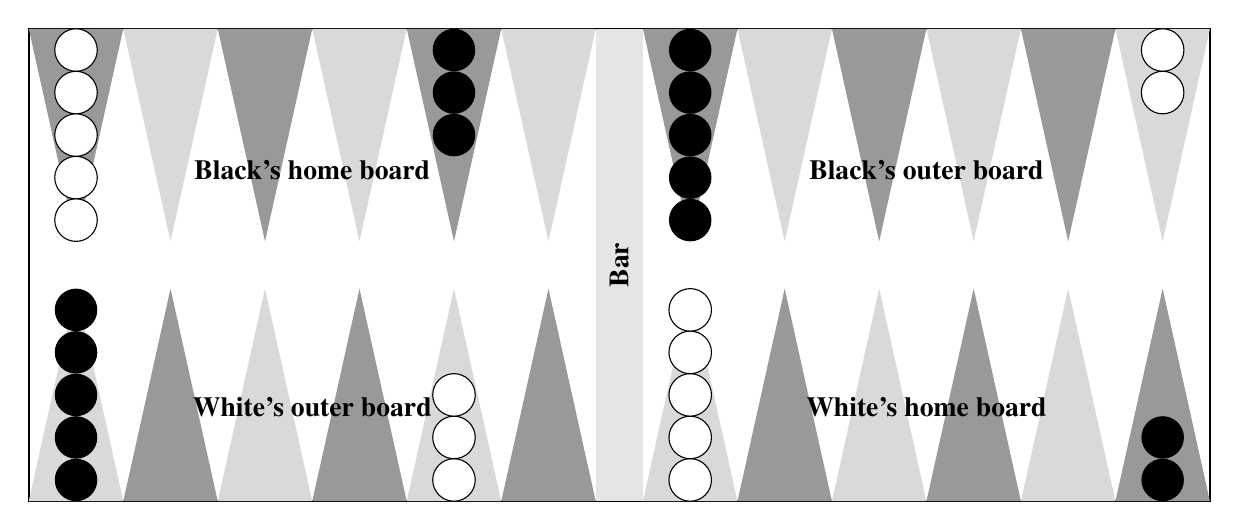
\begin{tikzpicture}[scale=0.3]
  % checker radius (in unscaled units)
  \def\r{0.9}

  % overall board
  \draw[thick] (0,0) rectangle (50,20);

  % the bar
  \fill[gray!20] (24,0) rectangle (26,20);
  \node[rotate=90] at (25,10) {\bfseries Bar};

  % bottom row of triangles (player side) — left half
  \foreach \i in {0,...,5} {
    \pgfmathsetmacro\x{4*\i}
    \fill[\ifodd\i gray!80\else gray!30\fi]
      (\x,0) -- (\x+4,0) -- (\x+2,9) -- cycle;
  }
  % bottom row of triangles (player side) — right half
  \foreach \i in {0,...,5} {
    \pgfmathsetmacro\x{26 + 4*\i}
    \fill[\ifodd\i gray!80\else gray!30\fi]
      (\x,0) -- (\x+4,0) -- (\x+2,9) -- cycle;
  }

  % top row of triangles (opponent side) — left half
  \foreach \i in {0,...,5} {
    \pgfmathsetmacro\x{4*\i}
    \fill[\ifodd\i gray!30\else gray!80\fi]
      (\x,20) -- (\x+4,20) -- (\x+2,11) -- cycle;
  }
  % top row of triangles (opponent side) — right half
  \foreach \i in {0,...,5} {
    \pgfmathsetmacro\x{26 + 4*\i}
    \fill[\ifodd\i gray!30\else gray!80\fi]
      (\x,20) -- (\x+4,20) -- (\x+2,11) -- cycle;
  }

  % --- starting checkers ---

  % Player (bottom) — white
  % 2 on 24-point → top, x-mid=48
  \pgfmathsetmacro\x{48}
  \foreach \j in {0,1} {
    \pgfmathsetmacro\y{20 - \r - \j*2*\r}
    \fill[white, draw=black] (\x,\y) circle (\r);
  }
  % 5 on 13-point → top, x-mid=2
  \pgfmathsetmacro\x{2}
  \foreach \j in {0,...,4} {
    \pgfmathsetmacro\y{20 - \r - \j*2*\r}
    \fill[white, draw=black] (\x,\y) circle (\r);
  }
  % 3 on 8-point  → bottom, x-mid=18
  \pgfmathsetmacro\x{18}
  \foreach \j in {0,...,2} {
    \pgfmathsetmacro\y{\r + \j*2*\r}
    \fill[white,draw=black] (\x,\y) circle (\r);
  }
  % 5 on 6-point  → bottom, x-mid=28
  \pgfmathsetmacro\x{28}
  \foreach \j in {0,...,4} {
    \pgfmathsetmacro\y{\r + \j*2*\r}
    \fill[white,draw=black] (\x,\y) circle (\r);
  }

  % Opponent (top) — black
  % 2 on 24-point → bottom, x-mid=2
  \pgfmathsetmacro\x{2}
  \foreach \j in {0,...,4} {    \pgfmathsetmacro\y{\r + \j*2*\r}
    \fill[black] (\x,\y) circle (\r);
  }
  % 5 on 13-point → bottom, x-mid=48
  \pgfmathsetmacro\x{48}
  \foreach \j in {0,1} {
    \pgfmathsetmacro\y{\r + \j*2*\r}
    \fill[black] (\x,\y) circle (\r);
  }
  % 3 on 8-point  → top, x-mid=32
  \pgfmathsetmacro\x{18}
  \foreach \j in {0,...,2} {
    \pgfmathsetmacro\y{20 - \r - \j*2*\r}
    \fill[black] (\x,\y) circle (\r);
  }
  % 5 on 6-point  → top, x-mid=22
  \pgfmathsetmacro\x{28}
  \foreach \j in {0,...,4} {
    \pgfmathsetmacro\y{20 - \r - \j*2*\r}
    \fill[black] (\x,\y) circle (\r);
  }

  % quadrant labels
  \node at (12,4)  {\bfseries White's outer board};
  \node at (38,4)  {\bfseries White's home board};
  \node at (12,14) {\bfseries Black's home board};
  \node at (38,14) {\bfseries Black's outer board};
  
  
  \end{tikzpicture}
    \caption{Backgammon board and starting positions of checkers}
    \label{fig:backgammonboard}
\end{figure}


% Setup
Each player begins with 15 checkers, which are placed on the board in a specific starting position, as shown in figure \ref{fig:backgammonboard}.
Checkers move in opposite directions towards their respective home boards (in figure \ref{fig:backgammonboard}, white moves anticlockwise and black moves clockwise).

% Objective
The objective of the game is for a player to move all 15 of their checkers into their home board and then bear them off (remove them from the board). 
The first player to bear off all their checkers wins the game.

% Starting the game
\subsection{Movement}
To start the game, each player rolls a die. 
The player with the higher number goes first and uses the numbers rolled by both players for their initial move. 
If they roll the same number, they roll again until different numbers appear.

% Turns
Players then alternate turns, rolling two dice at the beginning of each turn.

% Using the dice
A player must move their checkers according to the numbers shown on the dice. 
The two dice rolls represent two separate moves. 
For example, a roll of 5 and 3 (written as 5-3) means the player can move one checker 5 points and another checker 3 points, or move a single checker a total of 8 points (by moving it 5 points to an intermediate point, then 3 points further, or vice-versa), provided one of the intermediate landing points is not blocked by the opponent.

% Doubles
If a player rolls doubles (the same number on both dice), they can move four times the number shown on the dice. 
For example, a roll of 5-5 allows the player four moves of 5 points each (written as 5-5-5-5).

% Valid moves
A checker may only land on an open point, one not occupied by two or more opposing checkers. 
Points occupied by zero or one opposing checker are open. Any number of checkers of the same colour can occupy a single point.

If a player has legal moves available according to the dice roll, they must make them. 
If only one of the dice numbers allows a legal move, that move must be made. 
If either die allows a legal move but not both, the higher number must be played if possible. 
If neither die allows a legal move, the player forfeits their turn. 
If doubles are rolled and not all four moves can be made, the player must make as many moves as possible.

% Hitting
\subsection{Hitting and Re-entering}
If a checker lands on a point occupied by exactly one opposing checker (a blot), the opposing checker is hit and placed on the bar.
A player with one or more checkers on the bar cannot make any other moves until all their checkers on the bar have re-entered the game. 
A checker re-enters on the point in the opponent's home board corresponding to the number rolled on a die, provided that point is open. 
For example, if White has a checker on the bar and rolls a 3-5, they can re-enter on Black's 3-point if it is open, or on Black's 5-point if it is open. 
If neither corresponding point is open, the player forfeits their turn.

\subsection{Bearing off}
A player can only begin bearing off checkers once all 15 of their checkers are within their own home board.

A checker can be borne off a point if the number rolled on a die matches the point number (e.g., rolling a 4 allows bearing off a checker from the 4-point).
If a die roll is higher than the highest point on which the player has a checker, they may bear off a checker from the highest occupied point. 
For example, if a player rolls a 5 but has no checkers on the 5-point, but does have checkers on the 4-point, they can use the 6 to bear off a checker from the 4-point.

If a player can make a legal move using a die roll within their home board instead of bearing off, they are allowed to do so. However, if a checker can be borne off legally using a die roll, the player cannot choose to move a checker on a lower point if there are no checkers on points higher than the die roll. (The dice must be used to their highest possible value if possible, prioritising bearing off or moving from the highest points).

If a player's checker is hit while they are bearing off, they must re-enter that checker onto the bar and bring it back to their home board before they can resume bearing off.
\label{sec:rules}

\subsection{Backgammon Terminology}
TODO: not sure if i need this or should add to it
\begin{definition}[Blot]
A single exposed checker. Blots are disadvantageous as they can be hit.
\end{definition}

\begin{definition}[Hitting]
    The act of landing on a point occupied by a single opponent checker, sending the opponent's checker to the bar.
\end{definition}

\begin{definition}[Primes]
    A series of consecutive points that a player controls (with multiple pieces). Primes are effective at preventing an opponent from moving past.
\end{definition}

\begin{definition}[Anchors]
    A point in the opponent's home board occupied by two or more of the player's checkers.    
\end{definition}

\section{Existing Work}
\section{Game Design}
\section{AI and Games}

The development of AI for stochastic games has followed a separate path compared to deterministic games, due to major differences in the algorithms required. 
While traditional approaches for games like chess relied heavily on minimax search with alpha-beta pruning \cite{deepblue}, these techniques are less effective in games with chance elements due to the much larger branching factor when considering all possible dice rolls \cite{RussellNorvig}.

Early approaches to backgammon AI relied on evaluation functions created by backgammon experts and had limited depth lookahead \cite{berliner1980}. A significant breakthrough came with TD-Gammon, developed by Gerald Tesauro at IBM TODO, which used temporal difference learning (TD-$\lambda$) with a neural network to develop an evaluation function. TD-Gammon demonstrated that neural networks trained through self-play could learn complex decision making equal to world champions, without being explicitly programmed with backgammon specific strategies (Tesauro, 2002). TD-Gammon's success encouraged research in reinforcement learning and helped establish the application of neural network approaches for complex games (Sutton \& Barto, 2018).

\chapter{AI Algorithms and Architectures}
Before describing what techniques can be used to implement an AI system which plays backgammon, it is important to describe the game itself and the different types of AI systems that can be used to play it.
Backgammon is a two player, zero sum game with chance and perfect information.
Zero sum: One player's advantage is equivalent to the other player's loss. The sum of the players scores is always zero.
Perfect information: Both players have complete knowledge of the game state at all times. There is no hidden information.
Chance: The outcome of the game is not deterministic. The moves a player can make, and the outcome of the game depends on the rolls of the dice.

For such games, the best systems (such as AlphaGo) used a trained policy network, combined with Monte Carlo Tree Search (MCTS) in real-time gameplay \cite{aiparadigms}.
MCTS is limited to games with perfect information, and also requires that the action space is discrete, which are both true for backgammon.

This project includes different types of AI systems that can be used to play backgammon, such as rule-based systems, neural networks, and MCTS.

\section{Heuristics}
Heuristic approaches involve estimating the desirability of a given board state using rules which have been shown to work through trial and improvement. These rules typically combine several features based on expert knowledge, such as pip count difference (a measure of race progress), number of blots, strength of blockades (primes), and control of key points (anchors) [3, 5]. The agent then selects the move leading to the state with the best heuristic evaluation. While intuitive, designing effective heuristics can be complex, and heuristic rules may struggle with the nuances and dynamic nature of the game.

[3] Russell, S. J., \& Norvig, P. (2020). Artificial Intelligence: A Modern Approach (4th ed.). Prentice Hall. (Standard AI textbook covering game playing, search, RL).
[4] Campbell, M., Hoane, A. J., \& Hsu, F. H. (2002). Deep Blue. Artificial Intelligence, 134(1-2), 57-83. (Example of classical approach in chess).


\section{Stochastic Gradient Descent (SGD)}
While heuristic evaluation functions provide a computationally cheap way to estimate the strength of a board position, manually tuning the weights associated with different features can be challenging, subjective, and may lead to suboptimal performance. SGD offers a principled and automated method for learning these weights based on game experience.

The heuristic function $H(s, \boldsymbol{w})$ calculates the value of state $s$ as a linear combination of features $f_i(s)$ with corresponding weights $w_i$. The goal of SGD is to find the optimal weights $\boldsymbol{w}$ such that $H(s, \boldsymbol{w})$ gives the most accurate estimate for the value of being in a given state.

In the context of self-play, a common target is the final outcome $T$ of a game (e.g. +1 for a win and -1 for a loss). A loss function which measures the difference between the heuristic prediction and the target outcome can then be defined. A common choice for a loss function is the mean squared error (MSE):
$$
L(\boldsymbol{w}) = E[(T - H(s, \boldsymbol{w})^2]
$$
where $E[...]$ denotes the expectation over all possible states during the game.

The goal of SGD can be redefined as minimising the loss function $L(\boldsymbol{w})$.

Gradient descent algorithms work by iteratively updating the values of $\boldsymbol{w}$ by moving the values of $\boldsymbol{w}$ in the opposite direction of the gradient. This results in the following update rule:
$$
\boldsymbol{w} \leftarrow \boldsymbol{w} - \eta \nabla L(\boldsymbol{w})
$$
where $\eta$ is the learning rate, a value which determines the size of the steps the update rule makes.

The problem with this is calculating the gradient of the loss function requires summing over the entire distribution of states, which is computationally intractable. SGD overcomes this limitation by approximating the true gradient by estimating the gradient using only a few training examples at each step. This has the added benefit of helping to escape local maxima. TODO cite that paper in the other tab.

Over many iterations, these adjustments will move the weights $\boldsymbol{w}$ towards the value that minimises the prediction error, i.e. the heuristic function is as accurate as possible in predicting the value of a given state. [12] Bottou, L. (2010). Large-scale machine learning with stochastic gradient descent. Proceedings of COMPSTAT'2010, 177-186. (Provides a good overview of SGD for large-scale learning).


\section{Monte Carlo Tree Search}
Monte Carlo methods are a type of algorithm which estimates an unknown value based on random sampling. They are often used to solve problems that are deterministic in principle but difficult or impossible to solve with exact analytical methods TODO cite Russell and norvig. By generating many random samples and observing the outcomes, Monte Carlo methods utilise the Law of Large Numbers to approximate solutions.

TODO fun fact
The Law of Large Numbers states that the sample mean of $n$ independent and identically distributed random variables with mean $\mu$ approaches $\mu$ as $n$ tends to infinity.

Monte Carlo Tree Search (MCTS) is a Monte Carlo method which is used to search game trees to find optimal moves. Because of its stochastic nature, it is especially well suited to games which include chance, such as backgammon TODO cite [Browne, C. B., Powley, E., Whitehouse, D., Lucas, S. M., Cowling, P. I., Rohlfshagen, P., … \& Colton, S. (2012). A survey of Monte Carlo tree search methods. \_IEEE Transactions on Computational Intelligence and AI in Games, 4\_(1), 1-43.] 
TODO talk about minimax and how mcts approaches minimax

TODO cite https://link.springer.com/article/10.1007/s10462-022-10228-y
TODO talk about game trees in the AI and Games section as a definition. 
Intuition: A game tree is created with the current state as the root node. From then, random moves are made by all players until the end of the game (a leaf node) is reached, (or some other critieria is met such as TODO). The results of these games are propagated back throughout the tree and the value of each node is updated. By doing this a large number of times, the expected value of each node can be estimated, and the move resulting in the highest expectation can be picked.

The algorithm iteratively runs 4 steps until termination. 

\begin{enumerate}
    \item \textbf{Selection}: Starting at the root node, a child node is chosen according to a tree policy. This policy tries to balance exploring unvisited nodes (which may have high potential), with exploiting nodes which have been shown to be promising.
    \item \textbf{Expansion}: If the selected child node does not represent a terminal game state, it is then added to the stored game tree. 
    \item \textbf{Simulation}: From this newly added node, a simulation is run by randomly choosing moves for both players. This is continued until the end of the game is reached, or until another condition is met, such as reaching a move limit, or reaching a state where calculating the winner can be done easily.
    \item \textbf{Backpropagation}: The outcome of the game is backpropagated throughout the tree, from the expanded node to the root node. The statistics of each node along the path is updated, for example, the expected value of the node, and how many times the node has been visited. 
\end{enumerate}

This cycle is repeated until some condition is met. This could be until a certain amount of time has elapsed, or until some number of simulations has been reached. Finally, a move is chosen from the children of the root node, typically this is the node with the highest estimated value or the highest visit count.

There are many enhancements that can increase the performance of MCTS, many of which are described in "A Survey of Monte Carlo Tree Search Methods" \cite{Browne2012}. Some enhancements which are more applicable to backgammon are listed below.

\begin{itemize}
    \item One obvious improvement is to reuse trees that have already been computed previously. When an updated board has been passed to the algorithm, the grandchildren (because child nodes correspond to the opponent's turn; one more move something TODO to the player) can be checked. This will allow subsequent moves to have more accurate statistics on their child nodes, reducing wasted computation and allowing better moves to be chosen. Due to backgammon's large branching factor, it is important that the MCTS implementation can complete as many iterations as possible TODO too vague fix. If this is not the case, the likelihood of the grandchild node being computed will be low (or will have low N TODO). Due to the time taken searching the game tree for the grandchild, the agent will have less time to do further rollouts, which will result in worse performance.  

    TODO: A possible speed improvement was tested where the board was hashed and compared with the grandchildren. By creating a new tree rather than blah blah blah, improvement. however in practice, the branching factor resulted in there being very few common grandchildren. With the hashing and searching, this decreased the performance of the agent (where the agent was given 1 second to search). If the agent was given longer to search (thus resulting in a larger expanded game tree), it is possible that the performance would increase, as it would become increasingly more likely that a child had been explored.
    
    \item UCB1-Tuned \cite{6145622}: TODO cite  P. Auer, N. Cesa-Bianchi, and P. Fischer, “Finite-time analysis of the
    multiarmed bandit problem,” Mach. Learn., vol. 47, no. 2, pp. 235–256, 2002. One of the main problems in implementing Monte Carlo Tree Search is choosing the tree policy for selection. The tree policy needs to balance the exploration-exploitation tradeoff. UCB1-tuned offers a tigher bound compared with the more commonly used UCB1 algorithm TODO cite [8] Kocsis, L., \& Szepesvári, C. (2006). Bandit based Monte-Carlo planning. Proceedings of the 17th European Conference on Machine Learning, 282-293. When choosing which child node to explore, UCB1-tuned chooses the child which maximises the value.
    $$
    \mathrm{UCB} 1 \text{-Tuned}=\bar{X}_j+2C\sqrt{\frac{\ln n}{n_j} \min \left\{\frac{1}{4}, V_j\left(n_j\right)\right\}}
    $$ 
    where 
    $$
    V_j(s)=\left(1 / 2 \sum_{\tau=1}^s X_{j, \tau}^2\right)-\bar{X}_{j, s}^2+\sqrt{\frac{2 \ln t}{s}}
    $$ in the situation that child node $j$ has been chosen $s$ times in the first $t$ simulations, $\bar{X_j}$ is the average reward of child node $j$, $n$ is the total number of simulations, $n_j$ is the number of times node $j$ has been chosen already, and $C$ is a constant exploration parameter (where a higher value of C results in more exploration). 
    
    The first term $\bar{X_j}$ represents "exploitation", where a higher expected value will result in the node being picked more often, while the other term represents the "exploration" term, where values which have been picked a lower proportion of the time have a higher value.

    \item Rapid Action Value Estimation (RAVE): RAVE is a popular method for improving the information stored in each nodes statistics, particularly in Go programs which leads to faster convergence during the early stages of search \cite{GellySilver2007}. For each move, statistics across all simulations where that move appears is updated, with the assumption that a move that performs well in one particular is likely to perform well in other similar states. The RAVE and UCB values are then combined to estimate a nodes value.

    \item Combining MCTS with other models \cite{44806} \cite{Browne2012}: 
    One of the biggest improvements in MCTS is the integration of value networks to evaluate board positions, and policy networks to select moves. 
    By using a policy network, nodes with less value can be quickly identified and do not need to be expanded.
    By using a value network, games to not need to be expanded to the end.
    Instead the simulation is run to a predetermined depth, at which point the value network is used to evaluate the board position.
    Since the value network will be provided boards which are closer to the end of the game, it will be able to provide an accurate estimate of the value of the board position.
    This allows for more iterations of MCTS, increasing performance. The most notable example of this is AlphaGo, which used a combination of MCTS, policy networks, and value networks to achieve superhuman performance in Go, achieving a 99.8\% winrate against other Go programs \cite{44806}.

    
TODO definition: exploration-exploitation problem and what it entails / how it is applied in mcts. 
\end{itemize} 

Ross, Benjamin, and Munson present a closed form approximation for the probability that a player wins a backgammon race \cite{estimating}.
By using the Raw Pip Count (RPC) of each player, a Single Checker Model (SCM) is created is used to approximates each player's position as a single checker which needs to travel a distance equal to the RPC.
An existing approximation based on the central limit theorem in renewal theory is then used to estimate the SCM probabilities. 
After comparing this approximation to simulations of actual backgammon races, the formula was adjusted to account for bearoff rules and pip wastage, which the original SCM approximation did not take into account. This leads to the following value:
$$
\frac{\Delta^2 + \Delta / 7}{S - 25}
$$
where $\Delta = Y - X + 4$ is the adjusted difference in RPC between the two players, and $S = X + Y$ is the sum of the two players RPCs, where $X$ is the lower pip count, and $Y$ is the higher pip count of the two players. 
This value could then be compared with a precomputed lookup table to determine an approximate probability of winning the race (and therefore the game). 
This model was originally designed to be used by players to estimate the probability of winning during the game using only mental arithmetic, and therefore has a number of limitations. The model does not take into account hitting or any other interations, such as when a player is blocked, and some simplifications to the formula were made so players could easily calculate values mentally. 


TODO: define renewal theory and central limit theorem

----------------------------------------------
\section{Neural Networks} 

A neural network is a computational model which maps inputs to outputs using a series of transformations.
In particular, multilayer perceptrons (MLPs) model consists of an input layer, one or more hidden layers, and an output layer, where each layer is made up of interconnected nodes (neurons) that calculate a weighted sum of its inputs, and applies a non-linear activation function to produce an output. 
The universal approximation theorem states that a large enough MLP can approximate any continuous function to arbitrarily high accuracy \cite{Hornik1989}.
In the context of backgammon, the input layer would represent a board state, and the output layer would represent the probability of winning from that state.
In a deep neural network, only the board state is passed to the first layer, and the higher level features would be learned by the network as it is trained, however this required a large amount of training data and computation. 
A simpler approach is to use a network with less neurons and less layers, thus needing less training data and computation, and passing in the features of the board state as inputs (e.g. number of blots, number of anchor points, etc. TODO check if ive defined these above).

\section{Reinforcement Learning}

Reinforcement learning is a type of machine learning where an agent learns by interacting with an environment to maximise reward, as opposed to learning from labelled inputs and outputs (supervised learning) or learning from unlabelled data (unsupervised learning). By taking actions in an environment and observing the outcome, the agent is able to choose actions which maximise the reward.  
One technique for training an agent using reinforcement learning is to implement self-play, where the agent plays against itself and learns from the outcomes. 
As backgammon naturally has chance, the agent is forced to explore a wide variety of boards, which helps to avoid the problem of converging to a local minimum. 
This is unlike with stochastic gradient descent for two reasons: first, the neural network learns from every board state, while SGD learns only from the outcome; second, the neural network aims to learn the value of a board state, while SGD aims to learn a strategy for playing the game i.e. the neural network needs to see different positions to learn (which is natural to backgammon), while SGD needs to play against different styles to learn. 

From this, an initial model could be created which learns in the following way:
\begin{enumerate}
    \item The agent plays a game against itself, and the final outcome is recorded.
    \item The neural network is trained on every board state it has seen in the game, using the final outcome as the target value.
    \item The agent continues to play against itself and learn from the outcomes until some point is reached.
\end{enumerate}

The problem with this approach, is that by assigning each board state the same value, the implicit assumption is that all moves are equally important, which is not the case and causes the network to overestimate the value of early game states.
For example, if the agent wins a game but makes many mistakes along the way, the agent may reinforce the mistakes it made, as even bad states would be given a positive reward. 

To overcome this, temporal difference learning (TD learning) was developed, which was described by Sutton and Barto as "one idea central and novel to reinforcement learning" \cite{Sutton2018}.
The way TD learning overcomes this problem is by updating values at each time step based on the expected future rewards (multiplied by some factor $\gamma$), rather than just the final outcome. This comes with two main benefits:
\begin{itemize}
    \item By updating at every step, the agent is able to identify good and bad moves, and assign rewards accordingly.
    \item The agent is able to learn continuously after every action, rather than waiting until the end of a game to learn.
\end{itemize}
The reason expected future rewards are decayed by $\gamma$ is because rewards become less valuble the longer a player has to wait for them. 
This is because with longer wait times, the more variance there is in the outcome, and it is more likely that there will be errors. 
By having a decay factor, the agent is encouraged to take shorter, more certain paths to the goal.

This raises another problem, which is that initially during learning, only the states which lead to a win or loss have an associated reward, meaning learning can be extremely slow.
TODO this wording is shocking: The idea of TD-$\lambda$ is to solve this problem by updating the value of every past state in a sequence that led to the reward.
A value is chosen for $\lambda$ between 0 and 1, which determines the decay of the reward, with higher values giving more weight to states which are further away.
When a reward $x$ is received to a state $s$ at time step $t$, the value of previous states $s_{t-1}, s_{t-2}, ...$ are given a reward of $x (\lambda \times \gamma)^{t - i}$, where $i$ is how many steps back the state was seen.

Famously, TD-$\lambda$ was used in TD-Gammon \cite{Tesauro1995}, which was the first backgammon program to achieve expert level play.
It worked by using an MLP to predict the outcome of a game from the given board position. 
When making a move, the program would generate all legal moves from the current position, and use the network to evaluate each possible position.
The move with the highest predicted value was then chosen.

During training, the network started from a random initial state, and played against itself over and over. 
As training progressed, basic strategies began to emerge such as hitting blots, and creating anchors. 
TD-Gammon 1.0 contained 198 input nodes and 40 hidden units, and was trained for 200,000 games, resulting in an agent that was able to win regional tournaments.
TD-Gammon 2.1 was close to the world's best players, and was able to discover new strategies which changed how humans play certain board positions.
Pollack and Blair \cite{Pollack1997} argue that TD-Gammon's success was due to learning through self play, by showing a simpler model which learned effectively through the same method. 

TODO in the introduction talk about how AI in games helps create new AI techniques, which can be applied to other fields.

“TD-Gammon has definitely come into its own. There is no question in my mind that its positional judgment is far better than mine.
Only on small technical areas can I claim a definite advantage over
it . . . . I find a comparison of TD-Gammon and the high-level chess
computers fascinating. The chess computers are tremendous in
tactical positions where variations can be calculated out. Their
weakness is in vague positional games, where it is not obvious
what is going on . . . . TD-Gammon is just the opposite. Its strength
is in the vague positional battles where judgment, not calculation ,
is the key. There, it has a definite edge over humans . . . . In particular, its judgment on bold vs. safe play decisions, which is what
backgammon really is all about, is nothing short of phenomenal . . . .
Instead of a dumb machine which can calculate things much faster
than humans such as the chess playing computers, you have built
a smart machine which learns from experience pretty much the
same way that humans do”, Kit Woolsey, a top 10 world backgammon player, quoted in \cite{Tesauro1995}.



\section{Ensemble Models}
It is well established in psychology, economics, and other fields that although an individual may be inaccurate in their predictions, the average of many individuals is often more accurate than any one individual, a term referred to as the "wisdom of the crowd" TODO cite a bunch of people here.
This principle can be applied to machine learning, by creating an ensemble of models, where ntraining data is split between multiple models, and the predictions of each model are averaged to create a final prediction TODO cite Gavin Brown. Ensemble learning. In Encyclopedia of Machine Learning, pages 312 320. Springer, 2011. 

\chapter{Methodology}

This chapter describes the processes, techniques, and models used to design, implement, test, and evaluate the backgammon system.

\section{Overall System Design}
The system follows a three tier architecture, consisting of the presentation layer, application layer, and data layer. The presentation layer is responsible for the web client (implemented in React/TypeScript); the application layer consists of the game logic and AI (implemented in C++, Cython, and Python); and the data layer is responsible for the database (implemented SQLite). To interface between the presentation and application layer, a REST API is used to join and connect to a game, after which a WebSocket connection is established to allow for real-time communication between the client and server. To interface between the application and data layer, a Flask server, which uses SQLAlchemy as its ORM, manages database interactions.

By using a three tier architecture, the frontend, backend, and database can be developed independently. This allows for each layer to be tested and evaluated separately, while also allowing large architectural changes within each layer as long as the interfaces between layers remain constant. This proved useful when developing the AI, as some Python sections were replaced with languages which had higher performance. The three tier architecture also has security benefits; by forcing every request to flow through each layer, data can be controlled and validated. This stops clients from manipulating game states directly, preventing cheating and unwanted data manipulation.

There are however downsides to this architecture. The main downside is the increased complexity of the system, as there are more components to manage and maintain. Often this leads to similar code being written in multiple languages in different layers. For example, checks for a valid move are implemented in both the frontend and backend. This is discussed further in section \ref{sec:userinteractions}.  
Another downside is the increased latency of the system; where there is a barrier between layers, latency is naturally introduced. 

\section{Frontend Design}
TODO write out this idea: Chess is way more popular than backgammon, naturally this has led to popular chess websites being much more modern and better(?). Because of this, development of the frontend was heavily inspired by popular chess websites such as chess.com and lichess.org

Since chess has a much larger playerbase than backgammon, its online platforms have been developed much faster and more frequently. Websites like \href{https://www.chess.com/}{Chess.com} and \href{https://lichess.org/}{Lichess.org} were used to inspire development of the backgammon client, due to their modern, interactive interfaces.

\subsection{React and TypeScript}
The frontend, which is responsible for rendering the game board, handling user interactions, and communicating with the backend, was implemented in React/TypeScript. The frontend uses a REST API to join and connect to a game, after which a WebSocket connection is established to allow for real-time communication between the client and server. 

React/TypeScript was chosen for several reasons. React is the most popular frontend framework \cite{state_of_js_2024}, resulting in there being a large community and ecosystem, such as state management libraries (e.g. Redux) and UI component libraries (e.g. Shadcn).

TypeScript is a superset of JavaScript that adds static typing, which helps catch errors at compile time rather than runtime, and improves the developer experience by providing better autocomplete features. 
This is especially useful in a large codebase where the types act as documentation, helping to ensure that the code is more maintainable and less error-prone.


\subsection{Game Rendering}
The game board is rendered using Scalable Vector Graphics (SVG), which was chosen over other rendering methods, such as the HTML canvas element, as its format allows for easily manipulation of individual components on the board. This is useful for implementing features such as highlighting valid moves, showing the current player, and individual checker manipulation. As a vector format, SVG scaled perfectly across all devices and resolutions, increasing accessibility by being identical on all devices
Unlike canvas, SVG natively supports event listeners for clicking and hovering, and CSS animations can be easily added without requiring manual animation logic.
\subsection{Handling User Interactions}
\label{sec:userinteractions}
To allow for user preference, both drag-and-drop and click-and-move have been implemented. 
Drag-and-drop is implemented by using mouse event handlers (\verb|onMouseDown|, \verb|onMouseMove|, and \verb|onMouseUp|) to track the position of the mouse and update the position of the checkers accordingly. When checkers are clicked, coordinates of the mouse, the checker, and the board are used to determine the start and end positions of the move. A move is registered when the user releases the mouse, and the distance between the current checker and the closest triangle is less than a certain threshold. 
Click-and-move is implemented by using \verb|onMouseDown| to track the position of the checkers and update the position of the checkers accordingly. Generally, \verb|onClick| is used to handle user clicks, however \verb|onMouseDown| has many advantages over \verb|onClick|. Human computer interaction research \cite{mousedown1} \cite{mousedown2} has shown that responses under 100ms are perceived as instant. By using \verb|onMouseDown|, the time between a user's action and the system's response is greatly reduced, vastly increasing the perceived responsitveness of the system.

TODO talk about client side move validation

\subsection{Real time Communication}
When the user joins a game, they are connected to the server through a socket. This allows for real-time updates and allows the server to send messages to clients without the need for the client to make a specific request. The only alternative to this is some form of polling, where the client repeatedly requests updates from the server. This is inefficient leads to unnecessary latency and server load.

\section{Backend Design}

\begin{definition}[Object-Relational Mapping (ORM)]
Object-relational mapping is a technique used to convert data between an object oriented programming language and a database, allowing database interactions to be called directly.
\end{definition}

The backend is responsible for handling the game logic, state management, AI, and database interactions. The backend is implemented in Python using Flask for HTTP routing, Sockets for communication, and SQLAlchemy as an ORM to store and retrieve game states from an SQLite database. 
This layered design allows for the backend to be easily extended and modified, as each layer is responsible for a specific task. (game logic, AI, data handling).

\subsection{API Endpoints}
The server exposes a single REST endpoint to create games before handing off to WebSocket communication:

\textbf{POST /api/new\_game}: Generates a unique 5-character room code, instantiates a new \texttt{Board} in memory, which persists by being stored in the database. This allows for games to be resumed after a range of events, such as server restarts, or clients disconnecting. 

After initialization, all game actions, such as rolling dice, making moves, joining/leaving rooms—are handled over Socket events (Section~\ref{sec:room-management}).


\subsection{Room Management}
\label{sec:room-management}
Game sessions are tracked in a dictionary which is stored in memory and mapped to each game room by room code. The following Socket events are handled by the server:
\begin{itemize}
\item \texttt{join\_room}: Validates that the requested side is unoccupied, registers either a human (tracked by \texttt{sid}) or AI player (stores \texttt{ai\_model}), calls \texttt{join\_room(room\_code)}, and responds with the current board state via \texttt{"update\_board"}.
\item \texttt{leave\_room} / \texttt{disconnect}: Removes the client from the room, emits a \texttt{"left\_room"} event, and leaves residual state in the dictionary (to preserve ongoing matches during client disconnects).
\item \texttt{move}: Validates the move against the current board state, and if valid, updates the board, the corresponding board entry in the database, and emits and emits an \texttt{"update\_board"} event which sends the new board to all clients. If the move is invalid, an \texttt{"error"} event is emitted.
\item \texttt{roll\_dice}: Rolls the dice, updates the board, and emits an \texttt{"update\_dice"} event. This event sends the new dice values, invalid dice values, and valid moves to all clients in the room. 
If the player is an AI, the \texttt{ai\_move} function is called to handle the move asynchronously. This allows the AI to make its move, which can take substantial time and computation, without blocking the main event loop.
\end{itemize}
Turn enforcement: Every \texttt{move} or \texttt{roll\_dice} event compares the socket client's session id (SID) with the stored SID in the database. Unauthorised actions trigger an \texttt{"error"} event, preventing spoofed commands or out of turn moves.

When data is updated, the server emits events to clients. Clients listen for these events to stay synchronised with the server's game state.
The following socket events are emitted by the server:
\begin{enumerate}
    \item \texttt{joined\_room}: Emits a message to players that a new client has successfully joined the game.
    
    \item \texttt{update\_board}: After changes have been made to the board state, such as after dice rolls, player moves, AI moves, a new board is sent to players. 

    \item \texttt{update\_dice}: After a player rolls the dice, the updated dice is sent to all players.

    \item \texttt{error}: When an invalid action is attempted, such as an invalid move, or attempting to re-roll dice, an error is emitted to be displayed to players.
\end{enumerate}


\subsection{Database Schema and Interaction}
Persistence of game state is achieved through a single SQLAlchemy model, whose schema is shown in Figure~\ref{fig:game-schema}.

\begin{figure}[h]
\centering
\begin{tabular}{|l|l|l|}
\hline
\textbf{Column}             & \textbf{Type}          & \textbf{Description}               \\ \hline
\texttt{id}                 & Integer PK             & Primary key         \\ \hline
\texttt{room\_code}          & String(5), unique      & Game identifier                    \\ \hline
\texttt{positions}          & PickleType              & Board positions array   \\ \hline
\texttt{dice}, \texttt{invalid\_dice} & String(4)             & Current and invalid dice rolls     \\ \hline
\texttt{turn}               & Integer                & 1 = white to move, 0 = black      \\ \hline
\texttt{white\_bar}, \texttt{black\_bar} & Integer       & Checkers on the bar                \\ \hline
\texttt{white\_off}, \texttt{black\_off} & Integer      & Checkers borne off                 \\ \hline
\texttt{rolled}, \texttt{game\_over}  & Boolean        & Dice roll flag, game end flag      \\ \hline
\texttt{white\_ai\_model}, \texttt{black\_ai\_model} & String(20) & AI agent identifiers            \\ \hline
\end{tabular}
\caption{SQLAlchemy model schema}
\label{fig:game-schema}
\end{figure}

Two helper functions manage state transformations:
\begin{itemize}
\item Adding a board to the database: Creates and commits a new row, representing the initial state.
\item Updating a board in the database: Queries the latest row by room code, mutates its fields in place, and commits. One downside of this pattern is that intermediate states and moves are not stored, which could be useful for debugging or replaying games.
\end{itemize}

Atomic transactions and session management ensure that either all state changes occur together, preserving consistency. Queries always fetch the most recent state, guaranteeing that all clients operate on a synchronized game.

\section{Game Logic}
In this section, the core game logic is described, including the board representation, move generation and validation, and the interfacing between C++ and Python. C++ was used for the core game logic due to its performance advantages, which was then bound to Python using pybind11. 
\subsection{State Representation and Methods}
A \texttt{Board} class is used to store the game state, and contains the following attributes:
\begin{itemize}
\item \texttt{positions}: an array where each index corresponds to a point on the backgammon board. Positive values indicate the number of white checkers; negative values indicate the number of black checkers.
\item \texttt{white\_bar, black\_bar}: counters for checkers that have been hit and are waiting to re-enter.
\item \texttt{white\_off, black\_off}: counters for checkers that have been successfully borne off.
\item \texttt{dice}: captures the current roll.
\item \texttt{invalid\_dice}: stores the rolled dice values that are unusable in the current turn.
\item \texttt{valid\_moves}: stores every permissible sequence of moves for the active player in the current turn.
\item Game status flags: \texttt{rolled} (whether the dice have been rolled to prevent players from re-rolling dice), \texttt{passed} (whether all of one player's checkers have passed the opponent's checkers.  If this is true, no more pieces can be hit. ), \texttt{game\_over}, and \texttt{turn} (1 for White, -1 for Black).
\end{itemize}
The use of a single integer array to represent the board state allows for efficient storage and manipulation of the game state, as opposed to storing checker objects, which would increase memory usage and complexity with no significant benefit.

The following support methods are implemented to allow for easier implementation of AI agents:
\begin{itemize}
    \item \texttt{calc\_white\_left() / calc\_black\_left()}: computes a pip count (distance remaining) for each player by summing the product of checker count and point distance from bearing-off.
    \item \texttt{has\_passed()}: Determines passed status.
    \item \texttt{game\_over()}: returns true when either \texttt{white\_off} or \texttt{black\_off} reaches 15.
    \item \texttt{copy\_state\_from()}: copies a given board state into the current instance.
    \item \texttt{convert()}: serializes the entire C++ state into a Python dictionary (\texttt{py::dict}), allowing the Python layer to load and create database entries with minimal overhead.
    \item Clone and copy constructors: creates a copy of the board state, overriding the default python constructors, and allowing for exploration without altering the original state. This is useful for AI agents that need to explore multiple possible moves without modifying the original state.
\end{itemize}

\subsection{Move Generation and Validation}
As mentioned in section~\ref{sec:rules}, there are multiple rules on what moves can be made. Since each turn consists of moving multiple checkers, the move generation and validation process is complex. Each moving of a single checker cannot be checked individually, in the cases where a player has to maximise the number of checkers moved; or has to maximise the die used. Therefore, rather than checking each moves validity, a list of all possible moves is generated (which is also extremely useful for the AI agents).
The move generation process consists of two parts: identifying which dice can be used, then generating all possible moves.
\begin{enumerate}
    \item \textbf{Invalid Dice Detection}: Dice rolls that cannot be used to make any valid moves on the current board are first identified. Pseudocode for the function can be seen in algorithm \ref{alg:getInvalidDice}. A recursive helper function \texttt{evaluate\_dice()} is used to determine the unusable dice, as shown in algorithm \ref{alg:evaluateDice}. This function tries all possible ways to use the dice, applying one move at a time. If more dice can be used after a move, the function calls itself after removing the used dice from the list. If a point is reached where there are unused dice and no valid moves, the dice which result in the more dice being used, and higher value dice being used, are marked as valid, and the rest are marked as invalid. This can be extremely expensive, so optimisations are necessary. A very impactful optimisation is to return immediately if there is a single instance where all dice can be used. Since this is generally the case, this optimisation is very effective. 
    Once all invalid dice have been identified, the invalid dice are removed from the dice list and added to \texttt{invalid\_dice}.

    \item \textbf{Depth First Search for Move Sequences}: With invalid dice removed, a depth first search is performed on all the single die moves to create a list of full turn sequences, as shown in algorithm \ref{alg:getValidMoves}. Similarly to the invalid dice detection, a recursive helper function \texttt{dfs()} (as shown in algorithm \ref{alg:dfs}) is used to recursively generate all possible moves. In the general case, the function calls \texttt{get\_single\_moves()} (as shown in algorithm \ref{alg:singleMoves}) to list every legal single move that can be made from the current board state. For each of these moves, the function clones the current board state, applies the move, and removes the used die from the list. The \texttt{dfs()} function then calls itself with the new board state and the remaining dice. This process continues until all there are no dice remaining (base case), or no further moves can be made. For the base case, if all dice have been used, the function returns the list of moves it has calculated.
\end{enumerate}

\begin{algorithm}[H]
    \caption{Get Invalid Dice}
\label{alg:getInvalidDice}
    \begin{algorithmic}
    \State \textbf{Input:} Current dice list, board configuration
    \State \textbf{Output:} List of invalid dice
    \State \text{invalid\_dice} $\gets$ \text{dice}
    \State \text{max\_length} $\gets$ 0
    \State \text{max\_die} $\gets$ 0
    \State \text{board\_copy} $\gets$ \text{copy of board}
    \State
    \Comment{Attempt to use all dice in some order}
    \If{evaluate\_dice(board\_copy, dice, [], max\_length, max\_die, invalid\_dice)}
        \State \textbf{Return} [] \Comment{All dice are useable}
    \Else \Comment{Some dice are unusable and are removed}
        \State \text{result} $\gets$ invalid\_dice
        \For{each die in result}
            \State \text{remove the first occurrence of die from dice}
        \EndFor
        \State \textbf{Return} result
    \EndIf
    \end{algorithmic}
    
\end{algorithm}

\begin{algorithm}[H]
    \caption{Evaluate Dice} \label{alg:evaluateDice}
    \begin{algorithmic}
    \State \textbf{Input:} board, remaining\_dice, used\_dice, max\_length, max\_die, invalid\_dice
    \State \textbf{Output:} True or False
    \State
    \If{remaining\_dice is empty} \Comment{Base case where all dice have been used}
        \State \textbf{Return} True
    \EndIf
    \State
    \If{size(used\_dice) $>$ max\_length} \Comment{A new optimal set of dice has been found}
        \State max\_length $\gets$ size(used\_dice)
        \State invalid\_dice $\gets$ remaining\_dice
    \ElsIf{size(used\_dice) = max\_length and used\_dice is not empty}
        \State current\_max $\gets$ max element of used\_dice
        \If{current\_max $>$ max\_die}
            \State max\_die $\gets$ current\_max
            \State invalid\_dice $\gets$ remaining\_dice
        \EndIf
    \EndIf
    \State
    \If{size(remaining\_dice) = 1} \Comment{Move does not need to be played, only checked}
        \State die $\gets$ remaining\_dice[0]
        \For{each possible move on board using die}
            \If{move is valid}
                \State update max\_length, max\_die, invalid\_dice accordingly
                \State \textbf{Return} True
            \EndIf
        \EndFor
        \State \textbf{Return} False \Comment{There are no possible moves}
    \EndIf
    \State
    \For{each valid single move m on board using die}
        \State new\_board $\gets$ copy of board
        \State apply move m on new\_board
        \State new\_remaining $\gets$ remaining\_dice without the die that led to move m
        \State new\_used $\gets$ used\_dice plus die that led to move m
        \If{evaluate\_dice(new\_board, new\_remaining, new\_used, max\_length, max\_die, invalid\_dice) is True}
            \State \textbf{Return} True
        \EndIf
    \EndFor
    \State \textbf{Return} False
    \end{algorithmic}
\end{algorithm}

\begin{algorithm}[H]
    \caption{Get Valid Moves}
    \label{alg:getValidMoves}
    \begin{algorithmic}
    \State \textbf{Input:} board
    \State \textbf{Output:} List of valid moves
    \State
    \State valid\_moves $\gets$ empty list \Comment{Initialize the list for valid moves}
    \State board\_copy $\gets$ copy of Board \Comment{Create a copy of the current board}
    \State valid\_moves $\gets$ dfs(board\_copy, []) \Comment{Call DFS to find valid moves}
    \State \textbf{Return} valid\_moves \Comment{Return the list of valid moves}
    \end{algorithmic}
\end{algorithm}

\begin{algorithm}[H]
    \caption{Depth First Search (DFS) for Valid Sequences}
    \label{alg:dfs}
    \begin{algorithmic}
    \State \textbf{Input:} board, prev\_moves
    \State \textbf{Output:} List of valid sequences of moves
    \State
    \State \text{// If no dice left, return the one completed sequence (if any)} 
    \If{dice is empty}
        \If{prev\_moves is not empty}
            \State \textbf{Return} [ prev\_moves ] \Comment{Return the completed sequence of moves}
        \Else
            \State \textbf{Return} [] \Comment{Return an empty list if no moves were made}
        \EndIf
    \EndIf
    \State
    \State \text{// If exactly one die remaining, check for valid moves rather than making moves:} TODO make comments consistent
    \If{length(dice) == 1}
        \State results $\gets$ empty list \Comment{Initialize the list to store valid sequences}
        \For{each move in get\_single\_moves(min\_point)}
            \State results.APPEND(prev\_moves + [move]) 
        \EndFor
        \State \textbf{Return} results \Comment{Return the list of completed sequences with the one remaining move}
    \EndIf
    \State
    \State \text{// Otherwise, try every single move and recurse:}
    \State results $\gets$ empty list \Comment{Initialize the results list to store valid sequences}
    \For{each move m in get\_single\_moves(min\_point)}
        \State board\_copy $\gets$ copy of board \Comment{Create a copy of the current board}
        \State make move m on the board
        \Comment{Apply the move to the copied board} TODO remove minpoint
        \State sequences $\gets$ dfs(board\_copy, prev\_moves + [move]) \Comment{Recurse with the updated board and moves}
        \State results.EXTEND(sequences) \Comment{Add the resulting sequences to the final list}
    \EndFor
    \State \textbf{Return} results \Comment{Return the list of all valid sequences found}
    \end{algorithmic}
\end{algorithm}

\begin{algorithm}[H]
    \caption{Get Single Moves}
    \label{alg:singleMoves}
    \begin{algorithmic}
    \State \textbf{Input:} board, dice
    \State \textbf{Output:} Set of valid moves
    \State
    \State moves $\gets$ empty set \Comment{Initialize the set of valid moves}
    \State
    \If{ there are pieces on the bar}
        \For{each die d in dice}
            \If{die d can be used to re-enter}
                \State Add move corresponding to re-entering with die d to moves set
            \EndIf
        \EndFor
        \State // If there are checkers on the bar, re-entering is the only valid type of move. 
        \State // Therefore normal moves do not need to be checked, so the function can return early
        \State \textbf{Return} moves
    \EndIf
    
    \State
    \State \text{// normal moves} 
    \For{start in max(min\_point, 0) $\dots$ 23}
        \For{each die in dice}
            \State end $\gets$ start + die \Comment{Calculate the end position based on the die roll}
            \If{is\_valid(start, end)}
                \State moves.ADD( (start $\to$ end) ) \Comment{Add the valid move from start to end}
            \EndIf
        \EndFor
    \EndFor

    \State \textbf{Return} moves \Comment{Return the set of all valid moves}
    \end{algorithmic}
\end{algorithm}

\subsubsection{Executing Moves}
When a player chooses a move sequence, the engine proceeds as follows:
\begin{enumerate}
\item Validate the chosen sequence by checking if it is in \texttt{valid\_moves}.
\item Sequentially apply each move: decrement or increment \texttt{positions}, send hit checkers to the bar by incrementing \texttt{white\_bar} or \texttt{black\_bar}, and handle bearing off by incrementing \texttt{white\_off} and \texttt{black\_off}.
\item Remove corresponding dice values, by calculating the distance checkers have travelled. When bearing off, it is possible to bear off a checker from a point that is not equal to the die value, in which case the largest die is removed.
\item Recompute pip counts (\texttt{white\_left}, \texttt{black\_left}), update \texttt{passed} status, and detect \texttt{game\_over} if a player has borne off all pieces.
\item If no dice remain, or the player is forced to pass, the turn is swapped, \texttt{rolled} is set to false, and the dice are cleared.
\end{enumerate}


\subsection{Optimisations}
\paragraph{Pybind11}
Since board methods can be called millions of times during complex AI learning and play, it is important that they are as fast as possible. This resulted in the decision to write the board class in C++ (which is many times faster than Python), and bind it to Python using pybind11. By exposing  C++ class methods, significant performance improvements can be achieved, while maintaining the flexibility of Python for higher level logic, and still being able to use Python's extensive libraries for AI implementations.

\paragraph{Single die shortcut}
During the process of finding invalid dice and checking for valid moves, when there is only one die remaining, the function can return immediately after finding a move, rather than making the move and reaching the base case. As a result, all leaf nodes of the tree are not explored, and the function can prune these branches. Due to the large number of possible single moves, and the frequency of this case, this optimisation leads to significant performance improvements (approximately 67.5\% faster). The main reason this results in large speed improvements is the reduced number of deep copying, which is by far the most expensive primitive operation. 


\paragraph{Deep copying}
Often, the board state needs to be copied (e.g. to evaluate different moves), so that the original state is not modified. Especially during Monte Carlo Tree Search, this function can be repeated thousands of times per second, so it is important to reduce the cost of this operation. In Python, each attribute exists as a reference to a \texttt{PyObject}, rather than a data type such as an integer or array. This allows Python to be more flexible with its type restrictions, but also results in extremely expensive variable operations. When the board state is copied, every attribute must be allocated a new \texttt{PyObject}, and each element of the attribute (for lists) must also be checked for references to other sub-\texttt{PyObjects} (since everything is a \texttt{PyObject}). This results in many dynamic type checks, expensive memory allocations, and garbage collection cycles, despite types in the board being constant, and the size of the board being constant.

In contrast to this, C++ has a fixed type system, which results in elements being copied in far fewer operations, as data is stored contiguously rather than as references to separate memory locations. Without unnecessary type checks and garbage collection cycles, C++ is able to copy the board state much faster than Python, as shown in table \ref{tab:copy-times}. By overriding the default copy methods in Python with implementations in C++, the copy operation could be performed approximately 20 times faster.

\begin{table}[ht]
  \centering

  
  \begin{tabular}{@{}lS[table-format=2.3]@{}}
    \toprule
    {Operation}                  & {Time (s)} \\
    \midrule
    Python default \texttt{deepcopy}      & 16.916 \\
    Python overridden \texttt{deepcopy}   &  1.296 \\
    C++ default \texttt{deepcopy}         &  1.700 \\
    C++ overridden \texttt{deepcopy}      &  0.866 \\
    \bottomrule
  \end{tabular}
    \caption{State copy timings over 1 million iterations}
    \label{tab:copy-times}
\end{table}




\paragraph{Move Ordering Constraint} 
\label{sec:moveordering}
As described by Lishout et al. \cite{mctsinbackgammon}, a problem appears when calculating possible moves where identical positions can be generated through different sequences of moves, which is especially problematic when there are doubles. Rather than computing these positions and removing them, it is much faster to simply not compute them to begin with. 


Instead of naively exploring every ordered sequence of single moves, an ordering constraint on which points a checker can be moved to is implemented. After a checker is moved from point \texttt{i}, only subsequent moves where the starting point is greater than or equal to \texttt{i} are considered (less than \texttt{i} for black). This prunes many branches in the tree, particularly when doubles have been rolled, resulting in valid moves being calculated 5.9 times faster \footnote{This was tested by setting the dice of the same boards 10,000 times and recalculating valid moves. Unordered tree with repeated nodes: 10.935s. Ordered tree with unique nodes: 1.828s}.

Example: you have dice [2,4] and one checker on point 3 and another on 5.

Branch A: move from 3→5 (using the 2), then 5→9 (using the 4).

Branch B: move from 5→9 (4), then 3→5 (2).
Both end with one checker on 5 and one on 9—but in Branch B the second move would start at 3, which is < 5, so we skip it.

There are however, drawbacks to this optimisation, particularly for the users. When playing, they are also constrained by the move ordering constraint, leading to unintuitive behaviour and a poor user experience. 

While the optimisations were being tested, CProfile was used extensively to identify bottlenecks and measure speed improvements.


\section{AI Design and Architecture}
During the implementation of AI agents, multiple decisions were made, which are outlined in this section.


\subsection{Heuristic Agent}
\label{sec:heuristic}
The Heuristic Agent evaluates board positions as a linear combination of the following features, which were chosen based on backgammon strategy literature:
\begin{itemize}
    \item Difference in pip count
    \item Control of home, inner, and outer board
    \item Number of blots
    \item Length of the longest prime
    \item Number of checkers on the bar
\end{itemize}
Terminal states are handled by returning large constants ($\pm 1\times 10^6$).

In order to choose a move, the agent searches through all possible moves, evaluating each resulting state, and picks the move which corresponds to the highest value state. 

To improve the performance of the agent, stochastic gradient descent using self-play was used to find the optimal weights. The loss function was defined as 
\begin{equation}
    L(\mathbf{w})=E\left[(T-H(s, \mathbf{w}))^2\right]
\end{equation}
where $T$ is the target value (1 for a win, -1 for a loss), $H(s, \mathbf{w})$ is the heuristic value of the state $s$ with weights $\mathbf{w}$. 10,000 games were split into batches of 250 games, with the learning rate $\eta$ set to 0.01. 
The weights were updated using the Adam optimiser, which computes individual learning rates for each weight based on their individual gradients. 
Because the Adam optimiser accounts for momentum and bias-correction, it is often the best overall choice for an optimiser \cite{adam1}\cite{adam2}. 

\subsection{Monte Carlo Agent}
The Monte Carlo agent uses a time budgeted MCTS algorithm as described in section \ref{sec:mcts} to determine the best move to make. Users are able to choose between "fast", "standard", and "hard" agents, which have simulation time limits of 1 second, 5 seconds, and 10 seconds respectively. In the case that a double is rolled, the agent's time budget is doubled to account for the increased number of possible moves. The implementation of the MCTS agent is structured into two layers: the MCTS algorithm itself, responsible for selection, expansion, simulation, and backpropagation; and a higher level wrapper which is responsible for managing the game state, game tree, time management, and move selection.

In order to make the MCTS as fast as possible, Cython was chosen as the language to implement the MCTS algorithm, providing a balance of the performance C provides, and the flexibility of Python. Cython is a superset of Python which allows for C types and compilation, resulting in performance improvements. Simiarly to pybind11, by adding types to variables, Python is able to bypass certain type checks, and can allocate memory more efficiently. 
Although slower than a pure C++ implementation bound to Python using pybind11, Cython is able to call python functions and libraries, allowing MCTS to be combined with other models. 

\subsubsection{Move Selection and Initialisation}
When the agent is called, it is provided a copied instance of the board. In edge cases, where the agent has no moves, or only one move, the agent will return immediately. The agent then checks the current stored game tree for a matching node corresponding to the current board state. If a matching node is found, it is set as the root node, preserving statistics and child nodes. By using previously computed nodes, computation from previous iterations is not wasted. If a matching node is not found, the agent will create a new node with fresh statistics. The underlying MCTS algorithm is then called and runs for the specified time budget. 


Implementing move ordering from section \ref{sec:moveordering}, also results in much more accurate statistics. By forcing identical board positions, regardless of the move sequence which produced them, simulations are not split across duplicate nodes with the same board positions. As a result, each node has a higher visit count, improving the precision of its value estimates. 


\subsubsection{MCTS Algorithm}
While the MCTS algorithm is running, it continuously performs the four MCTS steps: selection, expansion, simulation, and backpropagation. The specific implementation details are as follows:
\begin{enumerate}
    \item \textbf{Selection}: The algorithm traverses the game tree, selecting child nodes based on UCB1-tuned, as described by equation~\ref{eq:ucb1}. By adjusting the exploration based on the variance of the outcomes, the agent is able to improve sample efficiency, especially in stochastic games such as backgammon. The best child node is continuously selected until a leaf node is reached. 
    
    \item \textbf{Expansion}: If the child is not terminal, it will have at least one unvisited child node. In this case, a random child node is selected and added to the tree.
    
    \item \textbf{Simulation}: A random playout is then performed until either a predetermined depth limit or a passed state has been reached. If the depth limit is reached first, one of three evaluations are used, based on the chosen evaluation mode:
    \begin{itemize}
        \item \textbf{Default}: The pip count ratio. e.g. if the white player has 10 pips and the black player has 20 pips, the ratio is $\frac{2}{3}$ for white and $\frac{1}{3}$ for black. This is a very fast evaluation, but not very accurate.
        \item \textbf{Heuristic}: The heuristic agent described in section \ref{sec:heuristic} is used to evaluate the board state. This is more accurate than only using the pip counts, but not as accurate as the neural network.
        \item \textbf{Neural Network}: The neural network described in section \ref{sec:neural} is used to evaluate the board state. This is the most accurate method, but requires a trained model.
    \end{itemize}
    The value from the evaluation is then normalised to a value between -1 and 1, where -1 is a loss for the player, 0 is a draw, and 1 is a win. 
    In the case that a passed state is reached, the $D^2/S$ formula is used to predict the winner. There are multiple benefits from this approach:
    \begin{itemize}
    \item By finishing the simulation early, the cost is reduced, allowing more simulations to be performed overall and increasing the accuracy of the statistics.
    \item Full playouts from passed positions involve random dice rolls, which may skew the results. By predicting the probability rather than relying on the law of large numbers, the value of the node has much lower variance.
    \item In a passed state, there are no more interactions between checkers. Random playouts through these positions result in very little strategic information, as the winner from this point is mostly determined by the pip count and chance. By using equation~\ref{eq:d2s}, the MCTS agent does not have to "re-learn" this relationship using repeated rollouts, and can instead directly use the precomputed statistic which it would eventually converge to.
    \end{itemize}

    \item \textbf{Backpropagation}: The result of the simulation is then backpropagated through the tree, updating the statistics of each node in the path. This includes the following values:
    \begin{itemize}
        \item $N$: The number of times the node has been visited.
        \item $Q$: The total reward the node has received.
        \item $Q^2$: The sum of the squares of the rewards received (used in the variance calculation).
    \end{itemize}
\end{enumerate}


\subsection{Neural Network Agent}
\label{sec:neural}
The Neural Network agent is a value function approximator, inspired by TD-Gammon \cite{Tesauro1995}, where the network predicts the probability that white wins a given board state. 
This was chosen as the method, as opposed to the network outputting a move, so the agent would not have to learn the rules of the game, and could instead focus on learning the strategy. The neural network was trained using TD-$\lambda$ learning in pytorch, which allows for strong GPU support and a familiar pythonic syntax.


\paragraph{Feature Representation}
Deep learning models are able to learn features from the raw input data, but in order to guide training, extra features were provided in the input. The following inputs were given to the network:
\begin{itemize}
    \item The number of checkers at each board position (positive for white, negative for black);
    \item The number of checkers borne off for each player;
    \item The number of blots for each player;
    \item The number of anchor points for each player;
    \item The length of the longest prime.
\end{itemize}

\begin{definition}[Vanishing Gradient Problem]
During backpropagation, the gradient of loss functions with respect to each weight is calculated. The gradients of some activation functions are always less than 1 (in the range of (0,1] for tanh and a maximum of 0.25 for sigmoid). The product of these values shrinks exponentially, resulting in earlier layers learning extremely slowly.   
\end{definition}

A multilayer perceptron was chosen where each layer is fully connected with ReLU activation functions. The output layer is a single neuron with a sigmoid activation function, which outputs a value between 0 and 1, corresponding to the probability that white wins. ReLU was chosen as it is extremely computationally cheap to compute and mitigates the vanishing gradient problem, since its derivative is always 1, ensuring that gradients being backpropagated do not shrink \cite{reluvanish}.

A sigmoid function was used in the output layer as its range is between 0 and 1, and is generally preferred for probability outputs \cite{LeCun2012}. 

\paragraph{Temporal Difference Learning}
Training was split into epochs of 500 games which were played concurrently. Despite dice rolls providing natural exploration, an additional exploration rate of 10\% was used, where the agent would pick a random move. 
After the games had been completed, TD-$\lambda$ learning was used to update the weights of the neural network, using a learning rate of $\eta$, and a $\lambda$ value which was provided to the agent at initialisation. A discount factor of $\gamma = 0.99$ was chosen as high values are preferred when applying TD=$\lambda$ learning to games. Using a high $\gamma$ value decreases the bias in the updates, but increases the variance, as the agent has to approximate future rewards at longer distances (i.e. the model is more complex) \cite{BRISCOE20112}. However, the high variance can be mitigated by increasing the number of games in the training data, whereas bias cannot be addressed in the same way, so choosing a model with low bias is less consequential.


An implementation which adjusted learning for momentum was used, however during testing, this was found to have a negative impact in the performance of the agent, as shown in figure TODO.
After each epoch, the neural network was evaluated by playing 500 games against a random agent, split evenly between playing as white and black. 
Once the learning process had been proved to work by being able to beat the random agent almost 100\% of the time, the heursitic agent was used instead of the random agent. Winrates from these evaluations were plotted to see how the agent was improving over time, with the weights being saved every 5 epochs. During training, the neural network was able to play and learn from approximately 4 games per second.

\subsection{Model Architecture Selection}

In order to determine what model architecture the final neural network




\chapter{Testing and Evaluation}
This chapter describes the testing and evaluation of the backgammon platform, covering both client and AI performance.
\section{Game Testing}
\paragraph{Unit testing}
Core game logic (e.g. move generation, dice handling, board updates) were validated using a suite of Python \texttt{unittest} cases. 
Each rule regarding movement, such as hitting, bearing off, and re-entry, each had multiple test cases, ensuring 100\% test coverage for game logic. 
Edge cases, such as forced passes (where a player is unable to move and gives up their turn) and forced moves, were also explicitly covered in the test cases.

\paragraph{Integration Testing}
Client-server interactions were tested using Selenium scripts which executed the following tasks:
\begin{enumerate}
    \item Create, join, and rejoin games via REST API;
    \item Establish socket connections and simulate human and AI players;
    \item Spectate AI vs AI games.
\end{enumerate}
Network interruptions and attempts to bypass client-side validation by sending requests directly to the server verified that the server emits appropriate errors.




\section{AI Agent Testing}
\subsection{Evaluation Framework}
\subsection{Performance Metrics}
\subsection{Neural Network Training Results}
\subsection{Tournament Results}

% \chapter{Testing and Evaluation}
\section{Game Testing}
\section{AI Agent Testing}
\subsection{Evaluation Framework}
\subsection{Performance Metrics}
\subsection{Neural Network Training Results}
\subsection{Tournament Results}


\chapter{Conclusion}
\section{Summary and Review}
\subsection{Project Achievements}
\subsection{Objectives Revisited}
\subsection{Key Challenges Faced}
\section{Limitations}
\section{Future Work}
\subsection{AI}
\subsection{Feature Additions}
\subsection{Deployment and Scalability}





%TC:ignore
\bibliographystyle{unsrtnat}
\bibliography{refs} 
%TC:endignore

\end{document}